% /chapters/4-group-actions/04-amoeba-trees.tex

\section{Amoeba trees}\label{sec:amoeba_trees}

Section~\ref{sec:recursive_constructions} concentrated on recursive constructions of amoebas with prescribed quantitative features, such as Fibonacci-type trees with high maximum degree.
This section turns to the structural side of the same subject and studies global amoeba trees through the interaction between automorphisms and feasible edge replacements.
The material is largely drawn from joint work in \cite{GomezetalPreprint}, which is in preparation as a paper at the time of writing; within this collaboration, the author proposed the section's central conjecture, discussed in Subsection~\ref{subsec:new_recursive}, that the \tFer group of every global amoeba tree has at most two orbits.

While Section~\ref{sec:recursive_constructions} produced concrete amoebas by recursive construction, the present section seeks general structural information about the relationship between $\Fer(T)$ and $\Aut(T)$.
Section~\ref{subsec:aut-trees-forests-unicyclic} develops the necessary background on automorphisms of trees, forests, and unicyclic graphs, the latter arising naturally as $T+f$ for $f\in E(T^c)$\footnote{Recall that $T^c$ denotes the \emph{complement} of $T$, that is the graph on the same vertex set obtained from flipping all of the adjacencies of $T$.}, i.e., as the unicyclic extensions whose automorphism groups generate elements of $\Fer(T)$.
Section~\ref{subsec:labelled-copies} then turns to the central question of when $A(T)$ is a normal subgroup of $\Fer(T)$, decomposing the canonical generators $\mathcal E_T$ in terms of automorphisms of $T$, of $T-e$, and of $T+f$, and showing that for trees the contribution from automorphisms of unicyclic extensions $T+f$ subsumes the others (Proposition~\ref{prop:tree-A-Aminus-in-Aplus}).

\emph{Throughout this section, all graphs are finite.}
The infinitary counterparts of several of the results presented here are discussed in Section~\ref{sec:infinitary_amoeba_graphs}.

\subsection{Automorphisms of trees, forests and unicyclic graphs}\label{subsec:aut-trees-forests-unicyclic}

For any graph $G$, we say $\varphi\in\Aut(G)$ \emph{fixes} the vertex $x\in V(G)$ if $\varphi(x)=x$, and that $\Aut(G)$ \emph{fixes} $x$ if every automorphism does.
A set $S\subseteq V(G)$ is \emph{fixed pointwise} (by either a single automorphism or by the entire group, respectively) if every element of it is fixed, and is \emph{fixed set-wise} by $\varphi$ if $\varphi[S]=S$.
Observe that $S$ is fixed set-wise if and only if $V(G)\setminus S$ is fixed set-wise.
An edge $xy$ is \emph{fixed} if the set $\{x,y\}$ is fixed set-wise.
Now let $xy$ be an edge of $G$.
If $\varphi\in\Aut(G)$ satisfies $\varphi(x)=y$ and $\varphi(y)=x$, then $\varphi$ is called an \emph{edge-inversion}.
In other words, an edge-inversion fixes the edge $xy$ but does not fix either of its endpoints.

The next lemma is a cornerstone result that we use throughout the section: automorphisms permute connected components.

\begin{lemma}\label{lemma:restriction-aut-component}
    Let $\varphi$ be an automorphism of $G$ and $C$ a connected component of $G$.
    Then $\varphi\restriction_C$ is an isomorphism between $C$ and a connected component (possibly $C$ itself) of $G$.
\end{lemma}

\begin{proof}
    If $\varphi[V(C)]=V(C)$, then the result is clear.
    Thus suppose that there is $v\in V(C)$ such that $\varphi(v)\notin V(C)$.
    Let $D$ be the connected component containing $\varphi(v)$.
    We claim that $\varphi[V(C)]=V(D)$.
    Indeed, given any $c\in V(C)$, a $cv$-path is preserved by $\varphi$, so there is a $\varphi(c)\varphi(v)$-path in $G$.
    Hence, $\varphi(c)\in V(D)$.
    The reverse containment holds because $\varphi^{-1}$ is also an isomorphism.
\end{proof}

\paragraph{Trees and forests.}

We begin by showing that any automorphism of a tree either fixes at least one vertex or inverts exactly one edge.

\begin{lemma}\label{lemma:aut-fixes-vertex-or-edge}
    Every tree $T$ has a vertex or an edge that is fixed by every $\varphi\in\Aut(T)$.
\end{lemma}

\begin{proof}
    Let $T$ be a tree and $L(T)\subseteq V(T)$ the set of \emph{leaves}, i.e., the vertices of degree $1$.
    Denote by $C(T)$ the \emph{centre} of $T$: the set of vertices $c$ for which $\varepsilon(c):=\max\{d(c,x):x\in L(T)\}$ is minimal among all vertices of $T$.
    Recall that every isomorphism is an isometry on the usual graph distance.
    Consequently, $C(T)$ is fixed set-wise by every $\varphi\in\Aut(T)$.

    It remains to argue that $C(T)$ consists of either a single vertex or two adjacent vertices, since then the conclusion follows from this and the preceding paragraph.
    Routine arguments show that whenever $T$ has more than two vertices, $T-L(T)$ is a tree with the same centre as $T$.
    For any tree $T$, $L(T)$ has at least two elements; thus, one can inductively remove all leaves from $T$ until there remains a tree of either one or two vertices, at which point the centre is the whole tree.
    But as argued, the centre is invariant under this operation.
    In other words, $C(T)$ consists of at most two vertices.
\end{proof}

For convenience, refer to an automorphism of a tree that fixes a vertex as a \emph{branch permutation} and use the symbol $\psi$ for it; for an automorphism that exchanges two adjacent vertices, use the letter $\varphi$ and call it an \emph{edge-inversion}, as defined above.
By Lemma~\ref{lemma:aut-fixes-vertex-or-edge}, every tree with non-trivial automorphism group has either a branch permutation or an edge-inversion.
The next corollary shows that the two conditions are mutually exclusive.

\begin{corollary}\label{cor:aut-tree-dichotomy}
    Every automorphism of a tree is either an edge-inversion or a branch permutation, and no automorphism is both.
\end{corollary}

\begin{proof}
    By Lemma~\ref{lemma:aut-fixes-vertex-or-edge}, it remains to show the exclusiveness.
    Since trees are acyclic, if $\varphi$ is an edge-inversion of a tree $T$ that inverts the edge $xy$, then every vertex in the connected component of $T-xy$ containing $x$ gets mapped to the connected component of $T-xy$ containing $y$.
    In particular, no such $\varphi$ has a fixed vertex.
\end{proof}

The procedure of iteratively removing leaves used in the proof of Lemma~\ref{lemma:aut-fixes-vertex-or-edge} also provides an algorithm for finding $C(T)$, and thus the vertex or edge fixed by the entire automorphism group, without computing any automorphisms of $T$.

\begin{definition}[Relative automorphisms]\label{def:relative-aut}
    Suppose that $H$ is an induced subgraph of $G$.
    The \emph{group of automorphisms of $H$ relative to $G$}, denoted $\Aut_G(H)$, is the set of automorphisms of $G$ that fix $V(G)\setminus V(H)$ pointwise.
    In symbols,
    $$
        \Aut_G(H):=\{\varphi\in\Aut(G):\varphi\restriction_{G-H}=\mathrm{id}_{G-H}\},
    $$
    where $\mathrm{id}_{G-H}$ denotes the identity map on $V(G)\setminus V(H)$.
\end{definition}

If $H$ is an induced subgraph of $G$, then $\Aut_G(H)$ is a subgroup of $\Aut(G)$ under composition.

\begin{lemma}\label{lemma:relative}
    The map $\Aut_G(H)\to\Aut(H)$ given by $\varphi\mapsto\varphi\restriction_H$ is a group monomorphism.
    Furthermore, if $V(H)$ is fixed set-wise by $\Aut(G)$, then $\Aut_G(H)$ is a normal subgroup of $\Aut(G)$.
\end{lemma}

The graph consisting of two disjoint triangles, taking $H$ to be one of them, gives an example where neither condition holds.

\begin{proof}
    Given $\varphi,\psi\in\Aut_G(H)$, by definition they agree on vertices not in $V(H)$.
    If they have the same restriction to $V(H)$, they agree on every vertex of $G$ and are therefore equal.
    This proves injectivity.

    Now assume that $V(H)$ is fixed set-wise by $\Aut(G)$, let $\varphi\in\Aut(G)$, and let $\psi\in\Aut_G(H)$.
    To prove normality, we show that $\varphi\circ\psi\circ\varphi^{-1}$ fixes every vertex of $V(G)\setminus V(H)$.
    Given $x\in V(G)\setminus V(H)$, the assumption implies that $V(G)\setminus V(H)$ is also fixed set-wise, so $\varphi^{-1}(x)\in V(G)\setminus V(H)$; the choice of $\psi$ then yields $\psi(\varphi^{-1}(x))=\varphi^{-1}(x)$.
    Hence $\varphi\circ\psi\circ\varphi^{-1}(x)=\varphi(\varphi^{-1}(x))=x$.
\end{proof}

The well-known result that the alternating group $A_n$ has no proper non-trivial normal subgroups for $n\geq 5$ \cite[Section~3.5]{dummit_foote_abstract_algebra}, combined with a check of small cases by hand, yields the following.

\begin{corollary}[Folklore]\label{cor:autT_is_not_An}
    If $T$ is a tree of order $n$, then $\Aut(T)$ is not isomorphic to $A_n$.
\end{corollary}

Now turn to the automorphisms of forests.

\begin{remark}\label{rmk:forest-aut-exchange}
    Let $F$ be a forest with connected components $T_1,\dots,T_k$, and let $\sigma\in\Aut(F)$.
    By Lemma~\ref{lemma:restriction-aut-component}, for each $1\leq i\leq k$ there exists $1\leq j\leq k$ such that $\sigma\restriction_{T_i}$ is an isomorphism from $T_i$ to $T_j$.
    Therefore, in addition to the automorphisms specific to each tree $T_i$, a forest also has automorphisms that exchange isomorphic components.
\end{remark}

Let $T$ be a tree and assume that $\psi\in\Aut(T)$ is a branch permutation that fixes a vertex $x$.
Let $T_1,\dots,T_k$ be the connected components of the forest $T-x$.
By Remark~\ref{rmk:forest-aut-exchange}, $\psi\restriction_{T-x}$ permutes these components by isomorphism, so the elements of $\Stab_{\Aut(T)}(x)$ induce a partition of the connected components of $T-x$ into classes of pairwise isomorphic trees, as depicted in Figure~\ref{fig:classes-of-tree}.

\begin{figure}[ht]
    \centering
    % figures/ex_type1.tex

\begin{tikzpicture}[
    % Style for the root node x (label now inside)
    rootNode/.style={
        circle, 
        draw=black, 
        fill=white, 
        very thick, 
        inner sep=0pt, 
        minimum size=7mm,
        font=\sffamily\bfseries\large
    },
    % Style for the small black child nodes
    childNode/.style={
        circle, 
        fill=black, 
        inner sep=0pt, 
        minimum size=1.8mm
    },
    % Connector lines
    edgeStyle/.style={
        draw=black, 
        line width=0.7pt
    },
    % Container shapes
    shapeStyle/.style={
        draw=black, 
        line width=0.7pt
    }
]

    % --- ROOT NODE ---
    \node[rootNode] (Vx) at (0, 0) {x};

    % --- CHILD NODES & SHAPES ---

    % 1. Left Square Node
    \node[childNode] (n1) at (-3.8, -1.5) {};
    \draw[shapeStyle, rotate around={45:(n1)}] ($(n1)+(-0.6,-0.6)$) rectangle ($(n1)+(0.6,0.6)$);

    % 2. Second Square Node
    \node[childNode] (n2) at (-2.3, -2.8) {};
    \draw[shapeStyle, rotate around={45:(n2)}] ($(n2)+(-0.6,-0.6)$) rectangle ($(n2)+(0.6,0.6)$);

    % Ellipsis between Squares
    \node[rotate=-45] at (-3.05, -2.15) {\(\dots\)};

    % 3. Third Node (Triangle)
    \node[childNode] (n3) at (0.2, -3.2) {};
    \draw[shapeStyle] ($(n3)+(0, 0.7)$) -- ($(n3)+(-0.7, -0.6)$) -- ($(n3)+(0.7, -0.6)$) -- cycle;

    % 4. Fourth Node (Triangle)
    \node[childNode] (n4) at (2.2, -2.4) {};
    \draw[shapeStyle] ($(n4)+(0, 0.7)$) -- ($(n4)+(-0.7, -0.6)$) -- ($(n4)+(0.7, -0.6)$) -- cycle;

    % Ellipsis between Triangles
    \node at (1.2, -2.8) {\(\dots\)};

    % 5. Right Ellipse Node
    \node[childNode] (n5) at (4, -1.3) {};
    \draw[shapeStyle] (n5) ellipse (0.75cm and 1.2cm);

    % --- EDGES ---
    \draw[edgeStyle] (Vx) -- (n1);
    \draw[edgeStyle] (Vx) -- (n2);
    \draw[edgeStyle] (Vx) -- (n3);
    \draw[edgeStyle] (Vx) -- (n4);
    \draw[edgeStyle] (Vx) -- (n5);

\end{tikzpicture}
    \caption{Components of $T-x$ partitioned into isomorphic classes by $\Stab_{\Aut(T)}(x)$.}
    \label{fig:classes-of-tree}
\end{figure}

Now consider an edge-inversion $\varphi$ of $T$, with $\varphi(x)=y$ and $\varphi(y)=x$ for some edge $xy\in E(T)$, and let $T_x$ and $T_y$ denote the two connected components of $T-xy$ that contain $x$ and $y$, respectively.
Applying Lemma~\ref{lemma:restriction-aut-component} to $\varphi\restriction_{T-xy}$ shows that $T_x$ and $T_y$ are isomorphic, as illustrated in Figure~\ref{fig:two-isomorphic-trees}.

\begin{figure}[ht]
    \centering
    % figures/ex_type2.tex

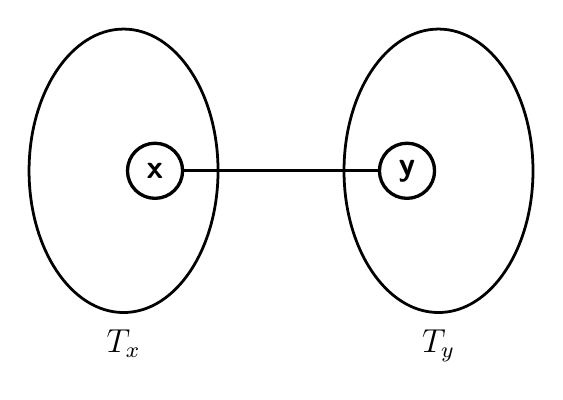
\begin{tikzpicture}[
    % Style for the vertices with labels inside
    vNode/.style={
        circle, 
        draw=black, 
        fill=white, 
        very thick, 
        inner sep=0pt, 
        minimum size=7mm, % Size adjusted for text
        font=\sffamily\bfseries\large
    },
    % Style for the set labels (Tx and Ty)
    setLabel/.style={
        font=\sffamily\bfseries\large,
        anchor=north
    },
    % Style for the edge
    edgeStyle/.style={
        draw=black, 
        line width=1pt
    },
    % Style for the container ellipses
    ellipseStyle/.style={
        draw=black, 
        line width=1pt
    }
]

    % --- COORDINATES ---
    \def\spacing{4} % Slightly wider spacing for the larger nodes

    % --- LEFT COMPONENT (Tx) ---
    \draw[ellipseStyle] (0,0) ellipse (1.2cm and 1.8cm);
    \node[vNode] (Vx) at (0.4, 0) {x};
    \node[setLabel] at (0, -1.9) {$T_x$};

    % --- RIGHT COMPONENT (Ty) ---
    \draw[ellipseStyle] (\spacing,0) ellipse (1.2cm and 1.8cm);
    \node[vNode] (Vy) at (\spacing-0.4, 0) {y};
    \node[setLabel] at (\spacing, -1.9) {$T_y$};

    % --- EDGE ---
    \draw[edgeStyle] (Vx) -- (Vy);

\end{tikzpicture}
    \caption{Components $T_x$ and $T_y$ of $T-xy$ are swapped by an edge-inversion.}
    \label{fig:two-isomorphic-trees}
\end{figure}

\paragraph{Unicyclic graphs.}\label{par:unicyclic}

Automorphisms of unicyclic extensions $T+f$ provide an important family of canonical generators of $\Fer(T)$.
We therefore record some structural facts about automorphisms of connected graphs with a unique cycle.

For this paragraph, $G$ is a connected graph with a unique cycle $C$.
For every $u\in V(G)$, denote by $G(u)$ the subgraph induced by the vertices $x$ for which there exists a $ux$-path that is edge-disjoint from $C$.

\begin{proposition}\label{prop:unicyclic}
    Let $\varphi\in\Aut(G)$ and $u\in V(C)$.
    \begin{enumerate}[label=(\alph*)]
        \item $\Aut(G)$ fixes $V(C)$ set-wise.

        \item $\Aut_G(C)$ is isomorphic to a normal subgroup of the dihedral group on $|V(C)|$ vertices.

        \item $\varphi[V(G(u))]=V(G(\varphi(u)))$.

        \item $\varphi\restriction_{G(u)}\colon G(u)\to G(\varphi(u))$ is a graph isomorphism.

        \item $G(u)$ is a tree on which $\Aut_G(G(u))$ has no edge-inversions.
    \end{enumerate}
\end{proposition}

\begin{proof}
    Part (a) follows from the fact that $\varphi$ is an isomorphism, so the image of $C$ must be a cycle of $G$; but $C$ is the only cycle in $G$.

    For (b), define $D$ as the image of the monomorphism from Lemma~\ref{lemma:relative} applied to $H=C$.
    The conclusion follows, with normality justified by (a).

    For (c), suppose that $x\in V(G(\varphi(u)))$.
    The automorphism $\varphi^{-1}$ preserves any $\varphi(u)x$-path and, by (a), preserves the property of being edge-disjoint from $C$, so $\varphi^{-1}(x)\in V(G(u))$.

    For (d), the restriction of an isomorphism is always an injective graph homomorphism, and by (c), the restriction is surjective.
    Now suppose that $x$ and $y$ are adjacent in $G-E(C)$.
    By (c), $\varphi^{-1}(x)$ and $\varphi^{-1}(y)$ both lie in $V(G(u))$, and since $\varphi$ is an isomorphism, they are adjacent.
    This proves that the restriction is an isomorphism.

    Finally, by the choice of $C$ and the observation that $G(u)$ is a connected induced subgraph of $G-E(C)$, $G(u)$ is a tree.
    By definition of $\Aut_G(G(u))$, $\psi$ fixes $V(G)\setminus V(G(u))$ pointwise; combined with (a), $\psi$ fixes $V(C)$ set-wise; since $\psi$ fixes $V(G)\setminus\{u\}$ pointwise, $\psi$ fixes $u$ as well.
    Being an isometry, $\psi$ must preserve the distance from any $x\in V(G(u))$ to $u$.
    But an edge-inversion fails to achieve this.
\end{proof}

For any tree $T$ and any $f\in E(T^c)$, the graph $T+f$ is unicyclic, so every element of $A(T+f)$ is subject to Proposition~\ref{prop:unicyclic}.
In Subsection~\ref{subsec:labelled-copies}, we show that these label permutations are canonical generators of $\Fer(T)$.

\subsection{Labelled copies, automorphisms and feasible edge replacements}\label{subsec:labelled-copies}

Recall from Subsection~\ref{subsec:fer} that for any finite graph $G$ on a label set $X$ with $|X|=n$, the following subgroup structure holds:
$$
    1\;\leq\; A(G)\;\bigl(\,\simeq\Aut(G)\,\bigr)\;\leq\;\Fer(G)\;\leq\; S_n.
$$
A natural question is: for which graphs $G$ is $A(G)$ a normal subgroup of $\Fer(G)$?
We divide the analysis into the connected and the disconnected cases.
In each case below, examples exist (so the cases are non-vacuous), though constructing them is more delicate than the reader might expect.

Except for trivial cases, $A(T)$ is a normal subgroup of $\Fer(T)$ only when $\Aut(T)$ is trivial.

\begin{proposition}\label{prop:local-amoeba-tree-asymmetric}
    Let $T$ be a local amoeba tree with at least three vertices.
    Then $A(T)$ is a normal subgroup of $\Fer(T)$ if and only if $T$ is asymmetric.%
    \footnote{A graph is called \emph{asymmetric} if its automorphism group is the trivial group.}
\end{proposition}

\begin{proof}
    Suppose that $T$ is a local amoeba tree on $n\geq3$ vertices and that $A(T)$ is normal in $\Fer(T)$.
    Since $T$ is a local amoeba, $\Fer(T)=S_n$.
    For $n=3$, the only tree is $P_3$, whose automorphism label group has order $2$ and is not normal in $S_3$, contrary to the hypothesis.
    For $n=4$, the only trees are $P_4$ and $K_{1,3}$, whose automorphism label groups have orders $2$ and $6$, respectively; neither is normal in $S_4$, again contrary to the hypothesis.
    We may therefore assume that $n\geq5$.
    The only normal subgroups of $S_n$ are then the trivial group $1$, the alternating group $A_n$, and $S_n$ itself; Corollary~\ref{cor:autT_is_not_An} rules out the second case, and the third case occurs only for complete and empty graphs.
    Since $T$ is a tree on at least three vertices, neither possibility applies, and thus $A(T)$ must be the trivial group.

    Conversely, if $T$ is asymmetric, then $A(T)\simeq\Aut(T)$ is the trivial subgroup, and thus normality holds immediately, regardless of the local amoeba assumption.
\end{proof}

\begin{proposition}\label{prop:A_eq_Fer}
    If $A(G)=\Fer(G)$, then exactly one of the following holds:
    \begin{itemize}
        \item $G$ is complete or empty; in either case, $G$ is a local non-global amoeba.
        \item $G$ has even order and is a perfect matching, that is, $G\cong\frac n2K_2$; in this case, $G$ is a global non-local amoeba.
    \end{itemize}
\end{proposition}

We do not know of any local amoebas $G$ for which $A(G)$ is the alternating group of order $|V(G)|$.

\begin{conjecture}\label{conj:disconnected-A-normal}
    If $G$ is a disconnected local amoeba for which $A(G)$ is normal in $\Fer(G)$, then either $G$ is asymmetric or an empty graph.
\end{conjecture}

For such a $G$, $\Fer(G)=S_X$ and so has only three normal subgroups.
If $A(G)$ is the trivial group, then $G$ is asymmetric; and if $A(G)=\Fer(G)$, then Proposition~\ref{prop:A_eq_Fer} implies that $G$ is empty.
The remaining case, $\Aut(G)\simeq A_n$, is open.

\paragraph{Labelled copies obtained from adding or removing a single edge.}

Recall that $\mathcal E_G$ consists of $A(G)$ together with all label permutations that witness a feasible edge replacement $(e\to f)$ of $G$, where $e\in E(G)$ and $f\in E(G^c)$.
By definition, $\Fer(G)=\langle\mathcal E_G\rangle$.

We are interested in three different ways to perform a feasible edge replacement $e\to f$ on a graph $G$: applying an automorphism of $G$ itself and then performing $e\to f$; first removing $e$, then applying an automorphism of $G-e$ and adding the corresponding $f$; and first adding $f$, then applying an automorphism of $G+f$ before deleting the corresponding $e$.
This motivates the following two sets of label permutations:
\begin{align*}
    A^+(G) &\;:=\;\bigcup_{f\in E(G^c)}A(G+f),\\
    A^-(G) &\;:=\;\bigcup_{e\in E(G)}A(G-e).
\end{align*}
Both sets are subsets of $S_X$, hence are well-defined as sets of label permutations of $V(G)$, since the graphs $G$, $G+f$, and $G-e$ share the same vertex set.

The following proposition shows the relationship between these sets and $\mathcal E_G$.

\begin{proposition}\label{prop:containment-automorphisms}
    For any graph $G$,
    $$
        A(G)\,\cup\,A^+(G)\,\cup\,A^-(G)\;\subseteq\;\mathcal E_G.
    $$
\end{proposition}

\begin{proof}
    By definition, $A(G)\subseteq\mathcal E_G$, so it suffices to handle the other two sets.

    Let $\sigma\in A(G+f)$ for some $f\in E(G^c)$, and let $\varphi_\sigma\in\Aut(G+f)$ denote the induced automorphism.
    Then $e:=\varphi_\sigma^{-1}[f]$ is an edge of $G+f$, so either $e\in E(G)$ or $e=f$.
    In the former case, Definition~\ref{def:G_sigma} gives
    $$
        E(G_\sigma)=\varphi_\sigma^{-1}[E(G)]=E(G+f)\setminus\{e\}=E(G-e+f).
    $$
    Hence $(e\to f)$ is a feasible edge replacement of $G$ with $\sigma\in\Fer_G(e\to f)$, so $\sigma\in\mathcal E_G$.
    If instead $e=f$, then $G_\sigma=G$, so $\sigma\in A(G)\subseteq\mathcal E_G$.
    This proves $A^+(G)\subseteq\mathcal E_G$.

    Now let $e\in E(G)$ and $\sigma\in A(G-e)$, with induced $\varphi_\sigma\in\Aut(G-e)$, and set $f:=\varphi_\sigma^{-1}[e]$.
    Then $f$ is not an edge of $G-e$: otherwise, applying $\varphi_\sigma$ would give $e\in E(G-e)$, a contradiction.
    If $f=e$, then $G_\sigma=G$, so $\sigma\in A(G)\subseteq\mathcal E_G$.
    Otherwise, $f\notin E(G)$, and
    $$
        E(G_\sigma)=\varphi_\sigma^{-1}[E(G)]=E(G-e)\cup\{f\}=E(G-e+f),
    $$
    so $\sigma\in\Fer_G(e\to f)$.
    Hence $\sigma\in\mathcal E_G$.

    Thus $A^-(G)\subseteq\mathcal E_G$, and all three inclusions hold.
\end{proof}

The following example shows that the inclusion in Proposition~\ref{prop:containment-automorphisms} is, in general, strict and that the corresponding generated groups also do not coincide.

\begin{example}\label{example:dif_groups}
    Let $G$ be the graph depicted in Figure~\ref{fig:Counterexample}.
    A direct analysis of the graph shows that $A(G)$ is the trivial group and that $A^+(G)$ and $A^-(G)$ are both equal to
    $$
        \bigl\{(0\ 1),\,(5\ 7),\,(0\ 6)(1\ 5)(2\ 4)(8\ 10)(9\ 11)\bigr\}.
    $$
    Hence $\bigl|\langle A(G)\cup A^+(G)\cup A^-(G)\rangle\bigr|=240$.
    On the other hand, $(v_1v_2\to v_7v_8)$ is a feasible edge replacement of $G$, and the permutation $\sigma:=(0\ 10\ 8\ 6\ 4\ 2)(1\ 11\ 9\ 7\ 5\ 3)$ satisfies $\sigma\in\Fer_G(v_1v_2\to v_7v_8)$.
    But $\sigma\notin\langle A(G)\cup A^+(G)\cup A^-(G)\rangle$.
    Moreover, $\Fer(G)=\langle\mathcal E_G\rangle\simeq S_{12}$.

    \begin{figure}[ht]
        \centering
        % figures/counterexample.tex

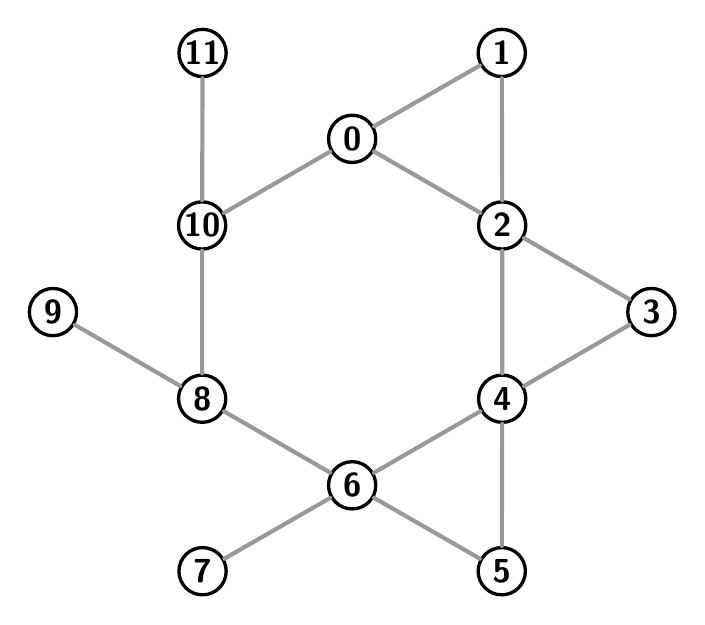
\begin{tikzpicture}[
    % Define the style for the vertices
    vNode/.style={
        circle, 
        draw=black, 
        fill=white, 
        very thick, 
        inner sep=0pt, 
        minimum size=6mm
    },
    % Define the style for the labels inside or near nodes
    vLabel/.style={
        font=\sffamily\bfseries\large
    },
    % Define the style for the connections
    edgeStyle/.style={
        draw=gray!80, 
        line width=1.5pt, 
        line cap=round
    }
]

    % --- COORDINATE DEFINITIONS ---
    % Central Hexagon Radius
    \def\hexR{2.2} 
    % Outer Nodes Radius
    \def\outR{3.8}

    % --- NODES ---
    % Inner Hexagon Nodes (0, 2, 4, 6, 8, 10)
    % Placed at 60-degree increments starting from 90 to keep it upright
    \foreach \i/\name in {0/0, 1/2, 2/4, 3/6, 4/8, 5/10} {
        \node[vNode] (V\name) at ({90 - \i*60}:\hexR) {};
        \node[vLabel] at (V\name) {\name};
    }

    % Outer Nodes (1, 3, 5, 7, 9, 11)
    % Placed between the inner nodes for symmetry
    \foreach \i/\name in {0/1, 1/3, 2/5, 3/7, 4/9, 5/11} {
        \node[vNode] (V\name) at ({60 - \i*60}:\outR) {};
        \node[vLabel] at (V\name) {\name};
    }

    % --- EDGES ---
    % Hexagon Ring
    \draw[edgeStyle] (V0) -- (V2) -- (V4) -- (V6) -- (V8) -- (V10) -- (V0);

    % Top Triangle (0-1-2)
    \draw[edgeStyle] (V1) -- (V0);
    \draw[edgeStyle] (V1) -- (V2);

    % Right Triangle (2-3-4)
    \draw[edgeStyle] (V3) -- (V2);
    \draw[edgeStyle] (V3) -- (V4);

    % Bottom Right Triangle (4-5-6)
    \draw[edgeStyle] (V5) -- (V4);
    \draw[edgeStyle] (V5) -- (V6);

    % The "Hanging" Edges (7, 9, 11)
    \draw[edgeStyle] (V7) -- (V6);
    \draw[edgeStyle] (V9) -- (V8);
    \draw[edgeStyle] (V11) -- (V10);

\end{tikzpicture}
        \caption{A graph $G$ for which $A(G)\cup A^+(G)\cup A^-(G)\subsetneq\mathcal E_G$.}
        \label{fig:Counterexample}
    \end{figure}
\end{example}

The next result shows that, when $G$ is a tree, the considerations simplify considerably: the canonical generators arising from automorphisms of $T$ itself, or from automorphisms of $T-e$ for $e\in E(T)$, are all expressible as products of canonical generators arising from automorphisms of unicyclic extensions $T+f$ for $f\in E(T^c)$.

We first need a lemma that refines the notion of branch permutation.

\begin{lemma}\label{lemma:median-tree-is-fixed}
    Suppose that $T$ is a finite tree, $u\in V(T)$, and $\varphi\in\Aut(T)$ is a branch permutation such that $\varphi(u)\neq u$.
    Then there is a vertex $c\in V(T)$ such that $\varphi(c)=c$ and $u,\varphi(u)$ lie in different connected components of $T-c$.
\end{lemma}

\begin{proof}
    A classical exercise in graph theory states that for any three vertices in a finite tree, there is a unique vertex $m$ lying on each of the three pairwise paths.

    Let $c$ be the vertex fixed by $\varphi$ closest to $u$, and apply the preceding fact to the triple $\{c,u,\varphi(u)\}$ to obtain $m$.
    Since $\varphi$ is an isometry on $T$, the graph distance satisfies
    $$
        d(u,m)\;=\;d(\varphi(u),\varphi(m))\quad\text{and}\quad d(m,c)\;=\;d(\varphi(m),c).
    $$
    Also, since $T$ is acyclic,
    $$
        d(\varphi(u),c)\;=\;d(\varphi(u),m)+d(m,c)
    $$
    and
    $$
        d(\varphi(u),c)\;=\;d(u,c)\;=\;d(u,m)+d(m,c),
    $$
    from where
    $$
        d(\varphi(u),m)\;=\;d(u,m)\;=\;d(\varphi(u),\varphi(m)).
    $$
    But both $\varphi(m)$ and $m$ lie on the path from $\varphi(u)$ to $c$; hence $\varphi(m)=m$.
    By the choice of $c$, $m=c$, which means that $c$ lies on the path from $u$ to $\varphi(u)$.
    Removing $c$ therefore disconnects $u$ from $\varphi(u)$, as claimed.
\end{proof}

\begin{proposition}\label{prop:tree-A-Aminus-in-Aplus}
    If $T$ is a tree with more than one edge, then
    $$
        \langle\,A(T)\,\cup\,A^-(T)\,\rangle\;\subseteq\;\langle\,A^+(T)\,\rangle.
    $$
\end{proposition}

\begin{proof}
    We first show that every involution in $A(T)$ lies in $A^+(T)$; the result for the generated group then follows from the fact that every automorphism of a tree is a product of involutions.

    Take a non-identity element $\sigma\in A(T)$ of order two and its induced automorphism $\varphi_\sigma\in\Aut(T)$.
    By Corollary~\ref{cor:aut-tree-dichotomy}, there are precisely two cases.

    \textbf{$\varphi_\sigma$ is a branch permutation.}
    Suppose that $\varphi_\sigma$ is a branch permutation.
    Since $\varphi_\sigma$ is non-trivial, there exists $u\in V(T)$ with $\varphi_\sigma(u)\neq u$.
    Let $c$ be the vertex of $T$ as in Lemma~\ref{lemma:median-tree-is-fixed}, so that $u$ and $\varphi_\sigma(u)$ lie in different components of $T-c$.
    The unique path between $u$ and $\varphi_\sigma(u)$ in $T$ passes through $c$, so $f:=u\,\varphi_\sigma(u)\notin E(T)$.
    Since $\varphi_\sigma$ has order two,
    $$
        \varphi_\sigma[f]\;=\;\varphi_\sigma(u)\,\varphi_\sigma^2(u)\;=\;\varphi_\sigma(u)\,u\;=\;f,
    $$
    so $\varphi_\sigma$ preserves the edge $f$.
    Combined with the fact that $\varphi_\sigma$ already preserves all edges of $T$, this gives $\varphi_\sigma\in\Aut(T+f)$, and hence $\sigma\in A(T+f)\subseteq A^+(T)$.

    \textbf{$\varphi_\sigma$ is an edge-inversion.}
    Now assume that $\varphi_\sigma$ is an edge-inversion, and let $xy\in E(T)$ be such that $\varphi_\sigma(x)=y$ and $\varphi_\sigma(y)=x$.
    Let $T_x$ and $T_y$ denote the connected components of $T-xy$ containing $x$ and $y$, respectively; observe that $\varphi_\sigma\restriction_{T-xy}$ is an automorphism of that exchanges connected components.
    Since $T$ has at least two edges and $T_x\simeq T_y$, each tree has at least one edge.
    Hence, we can pick some $u\in V(T_x)\setminus\{x\}$ and set $v:=\varphi_\sigma(u)$, so that $v\in V(T_y)\setminus\{y\}$ and, since $T$ is acyclic, $uv\notin E(T)$.
    Define $f:=uv\in E(T^c)$, and notice that $T+f$ is a unicyclic graph.
    Since $\varphi_\sigma$ preserves all adjacencies and non-adjacencies of $T$, and since $\varphi_\sigma^2=\id$ implies $\varphi_\sigma(v)=u$, we obtain $\varphi_\sigma[f]=vu=f$.
    Hence $\varphi_\sigma\in\Aut(T+f)$, so $\sigma\in A(T+f)\subseteq A^+(T)$.

    Therefore $\langle A(T)\rangle\subseteq\langle A^+(T)\rangle$.

    \medskip

    We next show that every involution in $A^-(T)$ lies in $A^+(T)$.
    Let $\sigma\in A^-(T)$ be of order two, and let $e=xy\in E(T)$ be such that $\sigma\in A(T-e)$.
    Set $F:=T-e$, a forest with exactly two connected components $F_x$ and $F_y$ containing $x$ and $y$, respectively.
    Then $\varphi_\sigma\in\Aut(F)$ either fixes each component set-wise (and then acts as a branch permutation or edge-inversion when restricted to each component) or exchanges them.
    In either case, $f:=\varphi_\sigma(x)\,\varphi_\sigma(y)\in E(F^c)$.

    If $f=e$, then $\varphi_\sigma$ preserves $e$ set-wise.
    Combined with the fact that $\varphi_\sigma$ preserves all edges of $F=T-e$, this gives $\varphi_\sigma\in\Aut(T)$, so $\sigma\in A(T)$, and the previous part places $\sigma\in A^+(T)$.

    Assume now that $f\neq e$.
    Since $E(T)=E(F)\cup\{e\}$, it follows that $f\notin E(F)$ and hence $f\notin E(T)$.
    Thus $T+f$ is a unicyclic graph, and we claim that $\varphi_\sigma\in\Aut(T+f)$.
    Indeed, if $ab\in E(F)$, then $\varphi_\sigma(a)\,\varphi_\sigma(b)\in E(F)\subseteq E(T+f)$; and $\varphi_\sigma[e]=\varphi_\sigma(x)\,\varphi_\sigma(y)=f$.
    Therefore $\varphi_\sigma$ preserves the edge set of $T+f$, and $\sigma\in A(T+f)\subseteq A^+(T)$.

    Combining both parts, $\langle A(T)\cup A^-(T)\rangle\subseteq\langle A^+(T)\rangle$, as claimed.
\end{proof}

The containment in Proposition~\ref{prop:tree-A-Aminus-in-Aplus} can fail if the generated groups are dropped: even when restricting to the two types of tree automorphisms, it is possible that $A(T)\not\subseteq A^+(T)$.
Figure~\ref{fig:counterexample_trees} shows examples of both cases.

\begin{figure}[ht!]
    \centering
    % figures/counterexample_trees.tex

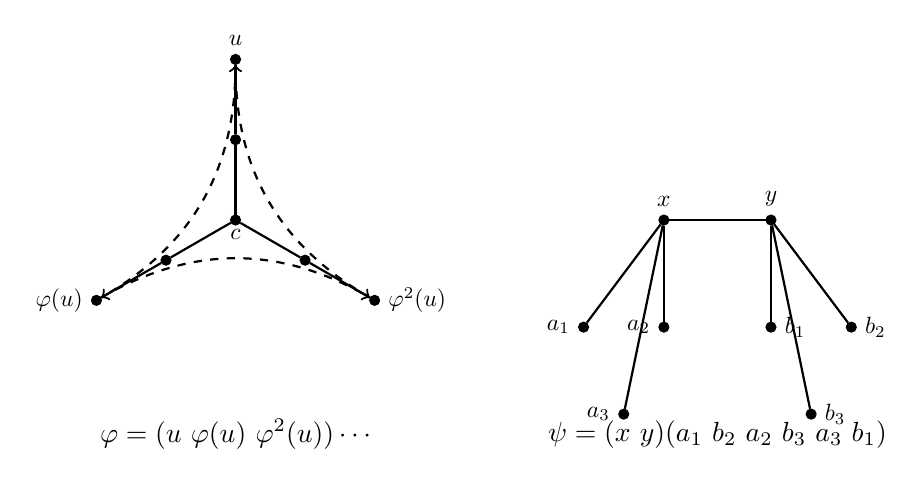
\begin{tikzpicture}[
    vertex/.style={circle, draw, fill=black, inner sep=1.5pt, minimum size=4pt},
    labeled/.style={circle, draw, fill=black, inner sep=1.5pt, minimum size=4pt, label={#1}},
    scale=0.85, every node/.style={transform shape}
]

% === Left tree: K_{1,3} with extended branches ===
\begin{scope}[shift={(-3.2,0)}]
    \node[labeled={[yshift=2pt]below:$c$}] (c) at (0,0) {};
    
    \node[vertex] (m1) at (90:1.2) {};
    \node[vertex] (m2) at (210:1.2) {};
    \node[vertex] (m3) at (330:1.2) {};
    
    \node[labeled={above:$u$}] (l1) at (90:2.4) {};
    \node[labeled={left:$\varphi(u)$}] (l2) at (210:2.4) {};
    \node[labeled={right:$\varphi^2(u)$}] (l3) at (330:2.4) {};
    
    \draw[thick] (c) -- (m1) -- (l1);
    \draw[thick] (c) -- (m2) -- (l2);
    \draw[thick] (c) -- (m3) -- (l3);
    
    \draw[->, dashed, thick, bend left=30] (l1) to (l2);
    \draw[->, dashed, thick, bend left=30] (l2) to (l3);
    \draw[->, dashed, thick, bend left=30] (l3) to (l1);
    
    \node[transform shape=false] at (0,-3.2) {$\varphi=(u\ \varphi(u)\ \varphi^2(u))\cdots$};
\end{scope}

% === Right tree: edge xy with 3 children each ===
\begin{scope}[shift={(4,0)}]
    \node[labeled={above:$x$}] (x) at (-0.8, 0) {};
    \node[labeled={above:$y$}] (y) at (0.8, 0) {};
    \draw[thick] (x) -- (y);
    
    \node[labeled={left:$a_1$}] (a1) at (-2, -1.6) {};
    \node[labeled={left:$a_2$}] (a2) at (-0.8, -1.6) {};
    \node[labeled={left:$a_3$}] (a3) at (-1.4, -2.9) {};
    
    \node[labeled={right:$b_1$}] (b1) at (0.8, -1.6) {};
    \node[labeled={right:$b_2$}] (b2) at (2, -1.6) {};
    \node[labeled={right:$b_3$}] (b3) at (1.4, -2.9) {};
    
    \draw[thick] (x) -- (a1);
    \draw[thick] (x) -- (a2);
    \draw[thick] (x) -- (a3);
    
    \draw[thick] (y) -- (b1);
    \draw[thick] (y) -- (b2);
    \draw[thick] (y) -- (b3);
    
    \node[transform shape=false] at (0,-3.2) {$\psi=(x\ y)(a_1\ b_2\ a_2\ b_3\ a_3\ b_1)$};
\end{scope}

\end{tikzpicture}
    \caption{Branch permutation (left) and edge-inversion (right) that are \textbf{not} elements of $A^+(T)$ for their respective tree $T$.}
    \label{fig:counterexample_trees}
\end{figure}

All of the above is finite by stipulation.
Section~\ref{sec:infinitary_amoeba_graphs} takes the same combinatorial setup, namely graphs with labelled vertices, the symmetric group on labels, and the \tFer group as a subgroup of $S_X$, into the descriptive-set-theoretic context, where $X$ is countably infinite and $S_X$ is a Polish group.
The structural questions of this section then translate into questions about Borel and analytic subsets of $S_X$, and the role of $A_n$ in the proof of Proposition~\ref{prop:local-amoeba-tree-asymmetric} is replaced by classification questions in descriptive set theory.

\subsection*{What lies beyond}

The forthcoming paper on which this section is based contains additional structural material, devoted to the study of the orbits of $\Fer(T)$ acting on $V(T)$ for a global amoeba tree $T$, and to the \emph{orbits graph} encoding the interaction between these orbits.
